\section{Introduction and Motivation}
\label{sec:introduction}
Twitter, as any other social network and blog, is a constant source of unstructured data that, if processed in the right way, can be leveraged to obtain valuable insights in several fields. Due to this reason, lots of companies have started to collect this huge amount of data in order to perform in-depth analysis on it; many of them have initiated to perform sentiment analysis to check customers satisfaction with respect to their products. Other organizations have started to use this asset, hereafter called Big Data, in their decision-making process that includes reporting, exploration of data and exploratory search (e.g., finding correlations). According to upGrad \cite{upGrad}, Big Data can help create pioneering breakthroughs for companies that know how to use it correctly.

A challenging aspect in Big Data analysis is to extract valuable insights that can drive business strategies and decisions. In this context, the social network Twitter plays a crucial role during the information retrieval phase: millions of people publish everyday short messages, hereafter tweets, that often contain their desires or demands. The aim of many companies is to leverage these tweets in order to catch common issues or demands to guide their business strategies for their products or services. These insights, according to upGrad \cite{upGrad}, can be used to develop new products/services, enhance marketing techniques, optimize customer service, improve employee productivity and find radical ways to expand brand outreach.

In addition to this, organizations aim also to intercept occasional issues or demands that are not constant over time but are very popular in a bounded period of time. This is the case when there is a sudden issue or request for a particular product or service that affects many customers. Catching this kind of insights, permits companies to better address their business short-term decision-making phase and enhance promptly their products or services. According to Ben Ridler \cite{customer-satistaction}, a business owner ability to effectively deal with customer complaints provides a great opportunity to turn dissatisfied customers into active promoters of the business.

Nowadays, according to \cite{twitter-stats}, there are more than 500 millions new tweets each day and this statistic is still growing every year. Thanks to this fact, many people have started to collect and group those tweets into datasets; many of them are easily and freely accessible by anyone through internet. Despite the fact that many of those datasets contain noisy data that force people to pre-process them, companies can elaborate those tweets in order to achieve the above mentioned business goals.

The aim of this project is to address in an efficient and effective manner the procedure of finding consistent topics over time inside tweet texts. In other words, the goal is to find topics that are frequent locally in a specific time frame but those topics, in order to be considered, must be frequent locally in a sufficient number of time frames. In this report are described in detail the solution to the just mentioned problem and the relative implementation. Finally, in Section \ref{sec:experimental_evaluation}, is presented an experimental evaluation of this project using the dataset described in Section \ref{sec:problem_statement} and \ref{sec:dataset} \cite{covid19-tweets-dataset}.

\section{Related work}
\label{sec:related_word}
In order to design and implement this project, several methods and techniques have been identified and implemented; anyway, there are some of them that have been implemented and widely tested but then discarded since they have not produced acceptable results to a possible final user during the experimental evaluation phase described in Section \ref{sec:experimental_evaluation}. In the first part of this section are described all those techniques used in order to pre-process the dataset, while in the second part are described all those methods used to find consistent topics over time using the pre-processed dataset. 

During the pre-processing phase of the dataset have been adopted several techniques widely used in natural language processing scenarios. The methods that have been implemented and kept in the final preprocessor script are described in details below and applied following this ordering:
\begin{enumerate}
	\item \textbf{Sentence segmentation}: the text string of each tweet is divided into sentences. In other words, the result of this step is a list composed by all the sentences that make up the tweet;
	\item \textbf{Tokenization}: with this technique, each sentence obtained from the previous step is split into even smaller parts called \textit{tokens}. In particular, has been used the blank character as string separator: due to this reason, a token corresponds to a word of the sentence;
	\item \textbf{POS Tagging}: this is the most complex task during the pre-processing of the dataset. The idea of the POS (\textit{Part Of Speech}) tagging technique is to assign to each token the corresponding tag (noun, verbs, adjectives, conjunction, etc.). The collection of tags used (tag set) can be considered as standard since it is used widely in the natural language processing community. In order to implement this technique, the map provided by the Python nltk library \cite{python-nltk} for English words has been used.
\end{enumerate}
The other technique used during the pre-processing phase of the dataset is an entity resolution method that is inspired to \textit{lemmatisation} \cite{lemmatisation-stemming}. The just mentioned technique aims to reduce the inflected form of a word in its canonical form in order to group together different words that have the same canonical form. The process implemented in this project is a simpler and non-automatic version of lemmatisation but still very effective on the given dataset \cite{covid19-tweets-dataset}. The goal is to define a set of \textbf{aliases} stored on the disk in a CSV file interpreted as a dictionary: if a word has an entry in that data structure, it will be replaced with its alias that represents a more general word (see Section \ref{sec:dataset} for further details).

\noindent Another technique that was initially implemented is \textbf{stemming} \cite{lemmatisation-stemming}. The aim of this method is to reduce the inflected form of a word in its root form (or "word stem") in order to group together words that have the same root form. The idea was to substitute the given word with its stem during the pre-processing phase. The major problem arose when the script to find the consistent topics over time has been run: the obtained results were not so meaningful since the root form of a word cannot be presented as a topic to the final user. Due to this reason and after many attempts to improve this approach, the just described technique has been abandoned.

In order to find out all the consistent topics over time, the major technique that has been used is the \textbf{frequent itemsets} mining method. The goal of this technique is to identify all the sets of items (in the context of this project, set of words) that appears together a sufficient number of times. In order to achieve the goal of this project, the association rules are not computed since they do not produce any valuable information. In a first attempt, the \textbf{A-Priori} algorithm \cite{apriori-algorithm} was used and implemented. The goal of this procedure is to find out initially frequent individual terms in the dataset and then extending the scope to larger item sets as long as those item sets appear sufficiently often in the database. The A-Priori algorithm leverages the contra-positive \textit{monotonicity} principle: if a word \textit{s} does not appear in \textit{N} sets, then no pair that includes \textit{s} can appear in \textit{N} sets.

\noindent A further attempt was to implement the PCY algorithm or its multihash variation \cite{pcy-multihash-algorithms}, but a more efficient technique that can be parallelized between many machines has been found: \textbf{FP-Growth} \cite{fpgrowth-paper}. The first step of this procedure, similarly to the A-Priori one, is to compute item frequencies and identify frequent items. Then, the second step of FP-Growth is to use a suffix tree structure, called FP-tree, to encode transactions without generating candidate sets explicitly, due to the fact that they are usually expensive to generate. When this second phase terminates the execution, the computed frequent itemsets can be extracted from the FP-tree. With the aim of speed-up the computation distributing the workload among different machines, a parallelizable version of FP-Growth has been used: \textbf{Parallel FP-Growth} \cite{pfpgrowth-paper}. This algorithm distributes the work of growing FP-trees based on the suffixes of transactions. Due to this improvement, it is more scalable than a single-machine computation.

\noindent The last technique used with the aim to improve the final result presented to the user is a variation of the \textbf{closed itemsets} method. The just mentioned technique must be executed after having identified all the frequent itemsets (when the PFP-Growth algorithm has terminated its execution) and its goal is to compact the final output. The idea of closed itemsets is that if there are two frequent itemsets where one is a subset of the other and they have the same frequency, the subset must be discarded. The method implemented in this project follows the same principle, but given two itemsets where one is a subset of the other, the subset is discarded only if it appears in as many time frames as the super set. If they do not appear in the same number of time frames, it means that probably they are different topics so they must be both kept in the result set. The frequency of appearance of the itemsets is not used as a discriminant parameter in order to decide whether to keep or not a subset of items due to the fact that, in any case, a topic composed by many items is much more meaningful than a topic with less items from the point of view of the final user.

\section{Problem statement}
\label{sec:problem_statement}
In order to achieve the goal described in Section \ref{sec:introduction} (i.e., identify consistent topics over time inside tweets), a public available dataset that groups more than 300.000 tweets that contain the hashtag \textit{\#covid19} \cite{covid19-tweets-dataset} has been used. As many other datasets composed of unstructured data dumped from a social network such as Twitter, this dataset has lots of fields that characterize each tweet (e.g., publisher's username, location and account information, text of the message, etc.). 

To identify consistent topics over time using those tweets, the only fields needed are the publication date of each of them and the relative text. In other words, in the working environment a tweet is defined as a tuple composed by the following fields:
\begin{itemize}
	\item \textbf{date}: the date of the tweet publication, expressed as an integer value that represents the number of seconds that have elapsed since the midnight of 1\textsuperscript{st} January 1970;
	\item \textbf{text}: the text of the tweet represented as a list of words. This list is obtained splitting the source text using the blank character " " as separator and processed as described in detail in Section \ref{sec:dataset}.
\end{itemize}

\noindent Therefore, in order to obtain the formal model of this problem, the following sets have been defined:
\begin{description}
	\item[TWEET] = the set of tweets, defined as $\mathrm{TIMESTAMP} \times \mathrm{TEXT}$ where $\mathrm{TIMESTAMP}\subset\mathbb{N}_{\geq 0}$ and $\mathrm{TEXT}=\{x | x \in \Sigma^*\}$ where $\Sigma$ is the reference alphabet;
	\item[TIMESPAN] = the set of all the possible time spans in which the input dataset can be split, defined as a subset of $\mathbb{N}$
	\item[TS-THRESHOLD] = the set of all the possible thresholds to identify frequent terms and topics in a single time span, defined as a subset of $\mathbb{N}_{\geq 0}$
	\item[GB-THRESHOLD] = the set of all the possible thresholds to identify consistent topics over all the time spans, defined as a subset of $\mathbb{N}$
\end{description}

\noindent The aim is to model an utility function \textit{f} defined as
\begin{center}
	\textit{f}: $\mathrm{INPUT} \mapsto \mathrm{TOPIC}$
\end{center}
where $\mathrm{INPUT}$ is defined as 
\begin{center}
	$\mathrm{TWEET} \times \mathrm{TIMESPAN} \times \mathrm{TS\-THRESHOLD} \times \mathrm{GB\-THRESHOLD}$
\end{center}
 and $\mathrm{TOPIC} = \{x | x \in \Sigma^*\}$ where $\Sigma$ is the reference alphabet. In other words, $\mathrm{TOPIC}$ is the set of all the possible consistent topics over all the identified time frames.

\section{Solution}
\label{sec:solution}
In order to design and implement an efficient solution to the problem shown in Section \ref{sec:problem_statement}, all the techniques described in the second part of Section \ref{sec:related_word} have been adopted. Those methods, however, has not been implemented using a naive approach (i.e., the frequent itemsets algorithm has not been executed over the entire dataset and then its results have been processed to reach the final result set). 

Since the goal is to find out consistent topics over time, the first piece of the solution is to identify all the necessary time spans in which the initial dataset has to be split. This has been achieved adopting a method that aims to be as flexible as possible not only with the provided dataset \cite{covid19-tweets-dataset}, but also with any other ones pre-processed with the procedure detailed in Section \ref{sec:dataset}. The developed algorithm takes as input two hyper-parameters: \textit{timespan} and \textit{timeunit}. The "timespan" parameter is an integer value greater than zero that identify how long would be considered a single time frame, while the "timeunit" parameter is a string that defined the unit of measure for which the "timespan" parameter has to be evaluated. In the actual solution, the possible time units supported are "day" and "hour"; anyway, other time units can be added quite easily modifying the script module that interpret those parameters and split the dataset entries. As an example, if the time span is set to 1 and the time unit is set to "day", the maximum difference between the timestamps of the last and the first tweet of each time frame would be less or equal than 86400 (i.e., the number of seconds in a single day). As a result of this first phase, it is obtained a list of time frames where each entry is itself a list of all the tweets included in that time frame.If the delivered script has been executed in debug mode, all the time frames that have been detected will be dumped with additional information in a separated text file. The just described procedure is shown in Algorithm \ref{split_dataset_algorithm}.

\begin{algorithm*}
	\caption{Split dataset by time frame}
	\label{split_dataset_algorithm}
	\begin{algorithmic}[1]
		\Function{split\_dataset\_by\_timeframe}{$dataset, timespan, timeunit$}
			\State $base\_timeframe\_item\gets None$
			\State $previous\_timestamp\gets None$
			\State $start\gets 0$
			\State $end\gets 0$
			\State $timeframes\gets []$
			\For{row in dataset}
				\State $actual\_timestamp\gets int(row[0])$
				\If{base\_timeframe\_item is None}
					\State $base\_timeframe\_item\gets actual\_timestamp$
					\State $previous\_timestamp\gets actual\_timestamp$
				\ElsIf{same\_timeframe(base\_timeframe\_item, actual\_timestamp)}
					\State $previous\_timestamp\gets actual\_timestamp$
					\State $end\gets end + 1$
				\Else
					\State $timeframes.append((start, end))$
					\State $start\gets end + 1$
					\State $end\gets end + 1$
					\State $base\_timeframe\_item\gets actual\_timestamp$
					\State $previous\_timestamp\gets actual\_timestamp$
				\EndIf
			\EndFor
			\If{start != end}
				\State $timeframes.append((start, end))$
			\EndIf
			\State \textbf{return} $timeframes$
		\EndFunction
	\end{algorithmic}
\end{algorithm*}

Then, for each time frame that has been identified, the frequent itemsets algorithm is applied. As a first attempt, was implemented the base A-Priori algorithm, optimizing the overall computation leveraging all the possible CPU cores splitting the workload among different processes (the number of processes to start would have been configurable hyper-parameter of the algorithm and initially, as default value, would have been set to four). This approach seems to be, even from the first stage of the project development, not a scalable solution since the overall computation has to be performed by a single machine. The problem was in turn exacerbated by the fact that the computation takes relatively long time to compute only the frequent pairs: computing all the super sets of frequent itemsets would have taken lot of computation time even in a multi-process environment. Due to these reasons, this initial solution was implemented and then discarded but it has been taken as "baseline method" during the evaluation phase of the delivered solution as described in Section \ref{sec:experimental_evaluation}.

The method applied in the delivered solution is the FP-Growth algorithm \cite{fpgrowth-paper}, briefly introduced previously in Section \ref{sec:related_word}. This procedure is widely supported in all the frameworks for massive data mining due to the fact that it is most efficient algorithm that can be executed in a cluster of machines to speed up the computation. More precisely, it has been used a parallelizable version of FP-Growth called Parallel FP-Growth, or simply PFP-Growth, as described in Section \ref{sec:related_word}. This algorithm, for each time frame, takes in input the following three parameters:
\begin{itemize}
	\item \textit{itemsCol}: the name of the column where the sets of items are located in the provided list. In the actual implementation, the sets of items are located in the "tweets" column;
	\item \textit{minSupport}: the minimum support for an itemset to be identified as frequent. In the actual implementation, this parameter is set to a constant value of 0.01 (i.e., 1\%). Then, the frequent itemsets for each time frame will be filtered later;
	\item \textit{minConfidence}: the minimum confidence for generating the association rules. Since for this task those rules are not needed, the parameter is set to a constant value of 0.6.
\end{itemize}

\noindent As soon as the PFP-Growth procedure has terminated its execution, the frequent itemsets are extracted from the result object and then filtered. With this post-processing filtering, the aim is to remove all the single-item frequent sets and all those frequent itemsets whose frequency is less than the support threshold (TS-threshold) decided by the user as described in Section \ref{sec:problem_statement}.

When all the frequent itemsets have been filtered for a single time frame, it is computed the maximal frequency value (i.e., how many times appears the most frequent itemset inside that time frame) and a global hash map that keeps track of all the frequent itemsets obtained among all the various iterations is updated. In other words, each frequent itemset is mapped into a list whose length is equal to the number of time frames and, initially, it is filled with "None" values. When the frequent itemset \textit{i} appears in the time frame \textit{s}, the list assigned to the itemset \textit{i} is updated in position \textit{s}. In particular, in position \textit{s} is assigned a float value that represents the weight of that topic on a scale between zero and one and then it is normalized in a scale between one and five. In other words, the importance of a consistent topic is computed as the normalized ratio between the frequency of the itemset \textit{i} and the maximal frequency value computed previously: if the importance is near one then the topic \textit{i} will not be considered as important, while if the importance is near five then the topic \textit{i} will be considered very important. The procedure just described is shown in detail in Algorithm \ref{find_frequent_topics_algorithm}.

\begin{algorithm*}
	\caption{Find frequent topics}
	\label{find_frequent_topics_algorithm}
	\begin{algorithmic}[1]
		\Function{find\_frequent\_topics}{$timeframes\_limits, dataset, ts\_threshold$}
		\State $frequent\_itemsets\_dict\gets \{\}$
		\State $tf\_id\gets 0$
		\For{start, end in timeframes\_limits}
			\State $tweets\_in\_timeframe\gets dataset.subset(start, end + 1)$
			\State $FPG\_results\gets FP-Growth(tweets\_in\_timeframe, minSupport=0.01, minConfidence=0.6)$
			\State \textit{Remove from FPG\_results itemsets with length 1 and itemsets with frequency less than ts\_threshold}
			\State $max\_freq\gets itemset\_most\_frequent(FPG\_results)$
			\For{item in FPG\_results}
				\State $key\gets item.itemset$
				\If{frequent\_itemsets\_dict not contains key}
					\State $frequent\_itemsets\_dict[key]\gets $ \textit{[None for i in range(num\_timeframes)]}
				\EndIf
				\State $values\gets frequent\_itemsets\_dict[key]$
				\State $values[tf\_id]\gets (4 * item.freq / max\_freq) + 1$
				\State $frequent\_itemsets\_dict[key]\gets values$
			\EndFor
			\State $tf\_id\gets tf\_id + 1$
		\EndFor
		\State \textbf{return} $frequent\_itemsets\_dict$
		\EndFunction
	\end{algorithmic}
\end{algorithm*}

As soon as the global hash map, hereafter \textit{frequencies\_dict} has been filled with all the results of every time frame, it has been leveraged in order to compute the consistent itemsets, hereafter topics, over time. As described in Section \ref{sec:problem_statement}, the algorithm has to be provided with a second threshold value called "global threshold" (GB-threshold) that tells in how many time frames a topic has to appear in order to be considered consistent over time. In order to achieve the goal, a new hash map called \textit{ranking\_dict} is used, where its keys are integer value and the relative value is a list: the key \textit{i} maps to a list that contains all the consistent topics that have appeared in \textit{i} time frames. All the frequent topics that have not appeared in a sufficient number of time frames (defined by the global threshold value), will be discarded. 

\noindent For each entry in the frequencies\_dict hash map, the list of weights is summarized as a single float value that represents the average weight. Then is created a tuple composed by the frequent topic and the relative average weight. Finally, that tuple is appended to the list associated to the number of time frames in which that topic appears in the ranking\_dict hash map as described above. 

When the ranking\_dict hash map has been built completely, it will start the final procedure for data manipulation. This latest part has been developed following a precise \textit{implementation choice}: a consistent topic that appears in few time frames is more important than a consistent topic that appears in many time frames. This choice has been taken since those consistent topics that appear frequently in many time frames would be also detected by any simple frequent itemsets algorithm, while the purpose of this project is different and the relevance of a topic not frequent in the entire dataset but very recurrent in few time frames is much more higher.

\noindent After that the above-mentioned implementation choice has been stated, the goal of this final procedure is to sort by frequency average weight the obtained entries of the ranking\_dict hash map. In order to follow the just described property, the ordering procedure starts from those consistent topics that appears in few time frames and then continues with those topics that appear in more time frames. This procedure will terminate its execution when all the frequent topics have been processed or when the maximum number of topics to show to the final user has been reached. Indeed, the user can specify with a hyper-parameter what is the maximum number of consistent topics over time that have to be shown when the overall procedure terminates. This feature aims also to speed up the computation in all those cases where the user has put a low TS-threshold value (i.e., there will be lots of frequent topics) since the just described procedure involves the ordering.

\noindent Furthermore, in the procedure just described is applied the variation of the closed itemset technique as mentioned in Section \ref{sec:related_word}. The aim is to remove all those subsets that appear in as many time frames as a super set and compact the output presented to the final user. This choice has been taken due to the fact that a topic composed by many words is much more meaningful with respect to a topic composed by less words. The just described procedure is shown in detail in Algorithm \ref{find_consistent_topics_over_time_algorithm}.

\begin{algorithm*}
	\caption{Find consistent topics over time}
	\label{find_consistent_topics_over_time_algorithm}
	\begin{algorithmic}[1]
		\Function{find\_consistent\_topics\_over\_time}{$frequencies\_dict, gb\_threshold, max\_topics\_to\_show$}
		\State $ranking\_dict\gets \{\}$
		\State $max\_key\gets 0$
		\For{key in frequencies\_dict}
			\State $n\_of\_non\_none\gets $ \textit{sum(x is not None for x in frequencies\_dict[key])}
			\If{n\_of\_non\_none >= gb\_threshold}
				\If{ranking\_dict not contains n\_of\_non\_none}
					\State $ranking\_dict[n\_of\_non\_none]\gets []$
				\EndIf
				\State $sum\_weights\gets 0$
				\For{entry in frequencies\_dict[key]}
					\If{entry is not None}
						\State $sum\_weights\gets sum\_weights + entry$
					\EndIf
				\EndFor
				\State $weight\_mean\gets sum\_weights / n\_of\_non\_none$
				\State $ranking\_dict\_value\gets ranking\_dict[n\_of\_non\_none]$
				\State \textit{ranking\_dict\_value.append((weight\_mean, key))}
				\State $ranking\_dict[n\_of\_non\_none]\gets ranking\_dict\_value$
				\If{n\_of\_non\_none > max\_key}
					\State $max\_key\gets n\_of\_non\_none$
				\EndIf
			\EndIf
		\EndFor
		\State $n\_topics\_already\_considered\gets 0$
		\State $actual\_key\gets gb\_threshold$
		\While{actual\_key <= max\_key and n\_topics\_already\_considered < max\_topics\_to\_show}
			\If{ranking\_dict contains actual\_key}
				\State $values\gets sort(ranking\_dict[actual\_key])$
				\State $new\_values\gets []$
				\For{topic\_tuple in values}
					\State $superset\_found\gets false$
					\For{topic\_to\_compare in values}
						\If{topic\_to\_compare.length > topic\_tuple.length and is\_superset(topic\_to\_compare.length, topic\_tuple)}
							\State $superset\_found\gets true$
						\EndIf
					\EndFor
					\If{not superset\_found}
						\State \textit{new\_values.append(topic\_tuple)}
						\State $n\_topics\_already\_considered\gets n\_topics\_already\_considered + 1$
						\If{n\_topics\_already\_considered == max\_topics\_to\_show}
							\State \textbf{break}
						\EndIf
					\EndIf
				\EndFor
				\State $ranking\_dict[actual\_key]\gets new\_values$
			\EndIf
			\State $actual\_key\gets actual\_key + 1$
		\EndWhile
		\State \textbf{return} $ranking\_dict$
		\EndFunction
	\end{algorithmic}
\end{algorithm*}

As a final step, the delivered procedure has to build an output file in order to present the obtained results to the final user. In order to achieve this goal, it has been used the matplotlib Python library \cite{matplotlib-python} that can be leveraged to produce a single PDF report file that contains all the graphs, one for each time frame that has been identified. With the aim to respect the implementation choice, the plots have been stored following that principle: the first plot contains all those consistent topics that have appeared in few time frames, the second plot contains all those consistent topics that have appeared in at least one more time frame with respect to the previous graph and so on. Furthermore, if the limit of items has been reached, the procedure will be stopped but the most relevant consistent topics are already stored in the final result set.

\noindent The type of plot is the horizontal histogram where on the Y axis there are the consistent topics and on the X axis there are the frequency weights on a scale between 1 (low frequency) and 5 (high frequency) and the topics are sorted from the most frequent (top) to the less frequent (bottom) in the relative number of time frames. The file name of the output file can be decided by the final user using a hyper-parameter or, if that parameter is not used, the output file would be "report.pdf".

\section{Implementation}
\label{sec:implementation}
In order to implement the delivered project, different tools have been used. First of all, the entire project has been developed using the Python 3 programming language due to the fact that it has many libraries freely available that help programmers to deal with huge quantity of data and process them in relatively easy manner using its natural language toolkit frameworks. Thanks to those libraries, it has been possible to develop and test many slight variation of the delivered solution with the aim to find the most efficient one in a relative short time. As a result, one of the many scripts that have been developed to compare the efficiency has been taken as a quite advanced "baseline method" during the experimental evaluation phase described in Section \ref{sec:experimental_evaluation}. 

The main external framework used during the development of this project is \textit{Apache Spark} \cite{spark-reference} in its version 3.0.1, a unified analytics engine for large scale data processing. Apache Spark is an efficient, fast and general purpose cluster computing framework with high-level APIs in different programming languages. Since it enables in-memory computations, Spark is way more efficient with respect to other frameworks that have been created for the same purpose, such as Apache Hadoop \cite{hadoop-reference}. The Apache Spark strength is that it provides many APIs that permits to parallelize the workload among all the cluster of machines in a really easy manner. Furthermore, Spark's APIs permits to access its data structures using SQL-like methods or using data-frame operations that are more or less the same as those ones exposed by the widely used Pandas Python library \cite{python-pandas}.

In order to integrate Apache Spark in the Python 3 script, the \textit{Pyspark} library \cite{pyspark-reference} has been used. Pyspark has been released in order to integrate Apache Spark and the Python programming language: it actually is a Python API for Spark. In particular, in order to support Apache Spark that has been written using the Scala programming language, Pyspark allows the Python interpreter to dynamically interface itself with the JVM (Java Virtual Machine) objects necessary for the script execution. This has been achieved using the Py4J library \cite{py4j-reference} that is inspired to the Java Remote Procedure Call standard. 

\noindent To implement the solution described in Section \ref{sec:solution}, two modules of Pyspark have been used: \textit{PysparkSQL} and \textit{MLlib}. The PysparkSQL module allows to apply SQL-like operations on a huge amount of structured or semi-structured data; indeed SQL queries can be used to manage its data structures. This module can be interfaced with several data sources such as Apache Hadoop, MySQL or Parquet and it can load even external data such as, for example, CSV or JSON files. Furthermore, this module introduces the DataFrame data structure, a tabular representation of structured data that is similar to that of a table from a relational database management system. Since all the datasets that will be used with the delivered solution are CSV files, the choice to use the PysparkSQL module has been quite obliged. In fact, the input dataset is immediately parsed and transformed into a Pyspark data frame object and all the operations of data manipulation are executed on that data structure due to the fact that those operations can be parallelized among different machines.

\noindent On the other hand, the MLlib module of Pyspark is a wrapper for the Spark's machine learning library and it leverages data parallelism techniques to store and deal with huge amount of data. The MLlib module supports many machine-learning algorithms for classification, regression, clustering, collaborative filtering, dimensionality reduction, and underlying optimization primitives. This module has been used due to the fact that it supports directly the PFP-Growth algorithm described in Section \ref{sec:solution} and it uses the same hyper-parameters already presented. As a point of strength, the MLlib module manages the parallelization on multiple machines itself, hence the developers do not have to implement also this feature.

The other tool that has played a crucial role during the development of the final solution is the nltk Python library (Natural Language ToolKit) \cite{python-nltk}. This module has been developed in order to deal in an efficient and effective way with human language data. Indeed, it has been used in order to parse and interpret the words of each tweet inside the given dataset. Furthermore, all the natural language processes described in Section \ref{sec:related_word} (sentence segmentation, tokenization and POS tagging) have been used thanks to the fact that the nltk library implements directly those procedures and it provides for free a POS tagging map for english words.

The third tool that has been used to build the delivered solution is the matplotlib Python library \cite{matplotlib-python}. This module has been used in order to present in a clear and concise manner the results obtained at the end of the script execution to the final user. In particular, the matplotlib library has been used to generate a single PDF file that contains several plots where each of them represents a subset of all the consistent topics over time that have been detected as described in details in Section \ref{sec:solution}.

The latest tool used in both dataset preprocessor script and in the consistent topics finder script is the atpbar Python library \cite{atpbar-reference}. The goal of this module is to show to the user a progress bar with the aim to inform the latter about the state of the execution progress and, in particular, how many tweets there are in the provided dataset and how many time frames have been identified. The strength of this library is that it can show to the user progress bars that are managed by different processes. Due to this fact, the final user will be always aware about the execution progress of all the scripts even if they have been executed in a multi process environment.

\section{Dataset}
\label{sec:dataset}
As described previously in Section \ref{sec:problem_statement}, in order to build and test the solution presented in Section \ref{sec:solution}, a public available CSV dataset with more than 300.000 tweets that contain the hashtag \textit{\#covid19} \cite{covid19-tweets-dataset} has been downloaded from kaggle.com and processed. As many other datasets that group together huge quantity of unstructured data, it had to undergo a pre-processing phase in order to remove unnecessary features and noisy data. 

In that dataset, a tweet is defined as a data item composed of thirteen features: \textit{user-name}, \textit{user-location}, \textit{user-description}, \textit{user-created}, \textit{user-followers}, \textit{users-friends}, \textit{user-favourites}, \textit{user-verified}, \textit{date}, \textit{text}, \textit{hashtags}, \textit{source}, \textit{is-retweet}. In order to achieve the goal described in Section \ref{sec:problem_statement}, only two features are needed: the publication date of the tweet and the relative text. Due to this reason, the first stage of the pre-processing consists to remove all the non-relevant data features. This has been achieved quite easily since the dataset is CSV (Comma Separated Value) file and the Pandas Python library \cite{python-pandas} has lots of APIs to manage efficiently such big datasets.

After this initial stage, each tweet has been processed singularly in a multi-process execution where to each process is assigned a portion of the input dataset. For each tweet in the dataset portion, each process has to manipulate both the date and the text fields in the following manner:
\begin{description}
	\item[Date] field is transformed into an UNIX timestamp. In particular the publication date is stored in the input dataset as a string formatted as "yyyy-mm-dd hh:mm:ss", but thanks to the \textit{datetime} Python library this transformation can be performed in a easy and fast way. With the aim to be complaint also with the format of another dataset that groups together tweets in order to perform sentiment analysis \cite{sentiment-analysis-dataset} described in Section \ref{subsec:test_dataset}, the script responsible for the date manipulation is capable to transform also dates formatted like "Mon Apr 06 22:19:45 PDT 2009" into a UNIX timestamp.
	\item[Text] field is transformed into a list of words. In particular, thanks to the \textit{nltk} \cite{python-nltk} Python library, the initial text has been split using the blank character " " as separator and only the useful words that can be leveraged in order to derive a topic have been kept. Due to this reason, only nouns and adjectives appear in the final result list. Furthermore, there are other situations where a word, even it is a name or an adjective, cannot be considered: 
	\begin{itemize}
		\item if the word contains a slash "/", non-ASCII characters or special Unicode sequences;
		\item if the word represents a numeric value;
		\item if the word is composed by only one character;
		\item if the word is a stop word. This method has been implemented because there are some words like "https" or "amp" that are tagged as nouns but they cannot be leveraged to build a topic.
	\end{itemize}
	As a note, if the preprocessor script has been executed in the debug mode, all the non-considerable words are dumped inside a separated CSV file (together with the relative timestamp) in order to check if the script cut off useful words. Then, each considerable word is filtered and sanitized in order to remove all the eventual noisy characters. In particular, the filtering method performs the following operations:
	\begin{enumerate}
		\item all the word's characters are lowered;
		\item all the emojis are removed;
		\item all the non-alphanumeric characters are substituted with a blank space (e.g., the word "white-house" is transformed to "white house");
		\item the word is split again using the blank character as separator to identify eventual other words after the previous operation;
		\item all the obtained words are rechecked again to see if they are considerable and, eventually, discarded;
		\item as a final operation, each of the obtained words are checked with an aliases map as described in Section \ref{sec:related_word}. If there is an entry for a word, then the associated value is substituted. The aim is to generalize as much as possible the words used inside the tweets leveraging the knowledge about that dataset in order to obtain better results: since all the texts contain the word "covid19" or one of its many variations (e.g., "sars-cov-2", "covid", "coronavirus", etc.), all of them are mapped to the word "covid19".
	\end{enumerate}
	After these filtering operations, a final check is performed over all the considerable words in order to find out if there are doubled words or empty string. 
\end{description}

When each process has terminated its execution, all the partial results are collected in a single list by the master process using a pipe-based communication and sort that list in ascending order using the timestamp field as key. The result is a list of tweets ordered by their publication: this feature can be leveraged by the main script described in Section \ref{sec:implementation} in order to lower the overall complexity. If the preprocessor script has been executed in debug mode, also the list that contains all the discarded words would be collected but not sorted.

As a final step, the result list has been converted by the master process in a Pandas \cite{python-pandas} data frame object and stored in a separated CSV file. The same procedure would be applied to the second list with all the discarded words if the preprocessor script has been executed in debug mode.

\section{Experimental evaluation}
\label{sec:experimental_evaluation}
In order to evaluate the quality of the solution and the relative results produced by it, both performance evaluation and a user validation of the final outcome have been adopted. The performance evaluation that has been done aims to take in consideration both execution time and memory usage, while the user validation involved several external people who have given a mark to the consistent topics produced by the solution described in Section \ref{sec:solution}.
For the experimental evaluation of the performances, the delivered script has been executed in an Apache Spark context composed by the following workers:
\begin{itemize}
	\item PC 1: two CPU cores (4 logical cores detected) with 6.8 GB of RAM available. It is also the Spark master process;
	\item PC 2: four CPU cores with 7.1 GB of RAM available.
\end{itemize}
Due to a problem not fully understood, the computation workload has not been distributed in any test on all the available workers, which have been configured properly and detected correctly by the Spark master. As a drawback, the performance evaluation that would have been carried out was not done in the desired way. To overcome this issue, a full implementation of the A-Priori algorithm has been considered as a first baseline method: this has been achieved using the mlxtend Python library \cite{mlxtend-reference} which exposes an already-implemented method for that algorithm. After different attempts, using both the dataset \cite{covid19-tweets-dataset} and the dataset described in Section \ref{subsec:test_dataset} \cite{sentiment-analysis-dataset}, has been noticed that the algorithm exceeds the main memory also with not too large datasets and it greatly reduces the performances, probably because of the many memory swaps. Due to this problem, the mlxtend library has been discarded and, as baseline method, has been considered a script developed for the same project that does not use the Apache Spark framework and implements a simplified version of the A-Priori algorithm to identify only frequent pairs. Even if the implemented algorithm is not a full version of A-Priori, the overall workload is distributed among different processes with the aim of leverage all the computation power of the single machine and consider it as a non-naive baseline. 

Executing the above-mentioned baseline algorithm distributing the workload among four processes, it takes few seconds less with respect to the delivered solution. In light of these results, some considerations need to be made:
\begin{itemize}
	\item as described above, in the delivered solution the workload has not been split across the machines, hence it has been executed locally (with almost 50\% CPU usage of PC 1);
	\item the delivered solution is a complete implementation while the baseline algorithm will find out only frequent itemsets of size 2 (i.e., frequent pairs).
\end{itemize}
Due to these reasons, the delivered solution seems to be more performing with respect the baseline method since it uses less CPU computation power and produces the final result as requested, even if it takes few seconds more. Make a comparison based on the memory usage had seemed to be quite impossible: the baseline method is fully implemented in Python, hence it is clear how many megabytes it is using in memory. But the delivered solution uses the Spark framework and all the computations that involves the Spark's libraries are carried by Java Virtual Machine, which does not expose in a clear manner how many megabytes in memory is using the delivered script. Due to this reason, an in-depth analysis of the memory consumption has not been made.

The other kind of experimental evaluation that has been performed in order to verify the effectiveness of the delivered solution is a validation of the obtained results (i.e., consistent topics over time) hearing the opinion of several people. To all of them have been presented the results obtained executing the delivered script using different hyper-parameters on both the provided dataset \cite{covid19-tweets-dataset} and the test dataset described in Section \ref{subsec:test_dataset} \cite{sentiment-analysis-dataset}. The most significant result on the first dataset have been obtained using a time frame of one day, a ts\_threshold value between 70 and 80 and a gb\_threshold value of 3: the results produced using these hyper-parameters have been evaluated with high marks since almost all the consistent topics detected are meaningful. Using a lower ts\_threshold value or a different gb\_threshold values seems to produce too many results and most of them are not meaningful from the point of view of the people interviewed. The most significant consistent topics over time that have been found in three time frames using the above mentioned hyper-parameters are shown in Figure \ref{fig:finding}.

\begin{figure*}[h!]
	\centering
	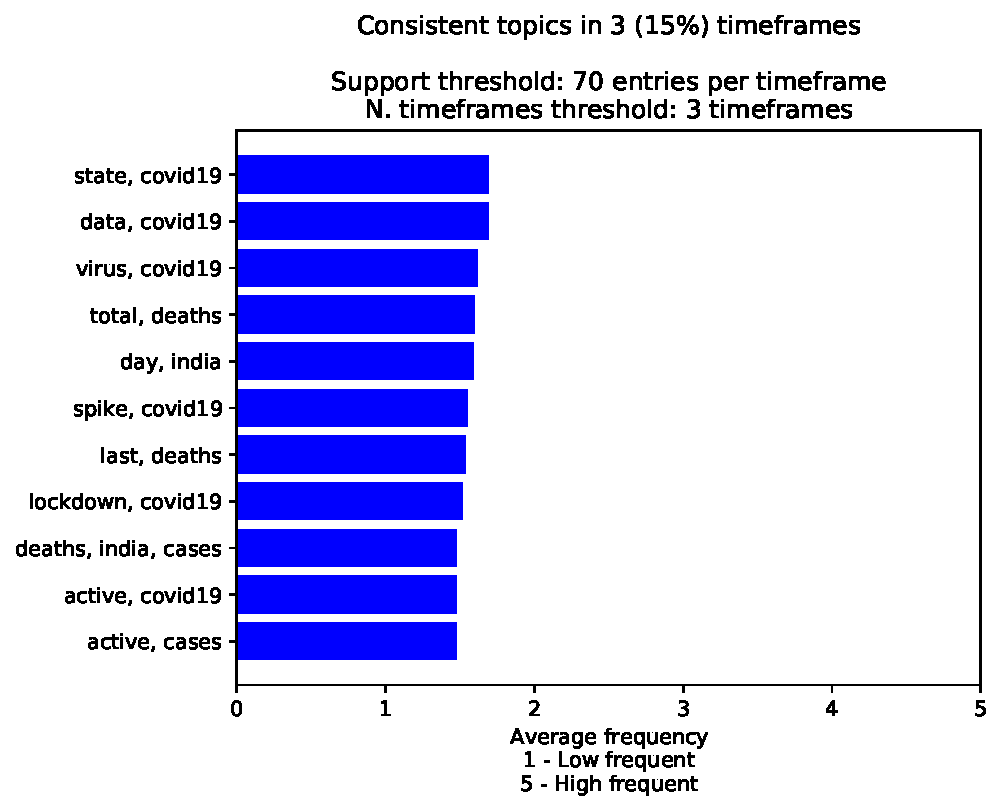
\includegraphics[width=0.8\linewidth]{images/findings.pdf}
	\caption{Most significant consistent topics over time found in three time frames}
	\label{fig:finding}
\end{figure*}

Furthermore, for the test dataset \cite{sentiment-analysis-dataset}, the most significant results have been obtained using a time frame of one day, a ts\_threshold value of 5 and a gb\_threshold value of 2: the number of results produced with these hyper-parameters is quite small but all of them have been marked highly by the people interviewed. Using lower values for the threshold seems to produce not too meaningful results and using higher values will produce almost no result using that dataset.

As a final check, the results of the delivered script have been compared with the output of the baseline method. Even if the latter will produce only the frequent pairs, its output is consistent with respect to the output produced by the delivered script. All the consistent topics that has been detected by the latter are composed by high-frequent pairs computed by the baseline method as expected.

\subsection{Test dataset}
\label{subsec:test_dataset}
In order to test the speed and the quality of the output produced by the delivered script, the dataset that groups more than 300.000 tweets that contain the hashtag \textit{\#covid19} \cite{covid19-tweets-dataset} has been used massively. This dataset has been already shown in details in Section \ref{sec:dataset}.

With the aim of perform a more in-depth analysis of the performances of the script, a bigger dataset has been uses: this dataset \cite{sentiment-analysis-dataset} contains 1.600.000 tweets extracted using the twitter API and they have been annotated in order to be used to detect sentiment. This dataset is stored in a CSV file where each item is composed by six fields: \textit{target} (the polarity of the tweet), \textit{ids} (tweet's id), \textit{date}, \textit{flag}, \textit{user} and \textit{text}. 

The most significant problem with using this dataset was during the pre-processing phase: the date field of each tweet was formatted using a not too handy format. As an example, the date of the first tweet was "Mon Apr 06 22:19:49 PDT 2009" and it has been quite hard to transform that date to a UNIX timestamp as required.

The other problem about this dataset is that it has not too many consistent topics over time, even if the quality of those detected by the algorithm described in Section \ref{sec:solution} is high. As a matter of fact, the hyper-parameters TS-threshold and GB-threshold has been set to, respectively, 5 and 2 in order to catch some consistent topics, while the dataset about covid19 \cite{covid19-tweets-dataset} those hyper-parameters have been set usually to, respectively, 70 and 3 as described in Section \ref{sec:experimental_evaluation}. 